% Options for packages loaded elsewhere
\PassOptionsToPackage{unicode}{hyperref}
\PassOptionsToPackage{hyphens}{url}
%
\documentclass[
]{book}
\usepackage{lmodern}
\usepackage{amssymb,amsmath}
\usepackage{ifxetex,ifluatex}
\ifnum 0\ifxetex 1\fi\ifluatex 1\fi=0 % if pdftex
  \usepackage[T1]{fontenc}
  \usepackage[utf8]{inputenc}
  \usepackage{textcomp} % provide euro and other symbols
\else % if luatex or xetex
  \usepackage{unicode-math}
  \defaultfontfeatures{Scale=MatchLowercase}
  \defaultfontfeatures[\rmfamily]{Ligatures=TeX,Scale=1}
\fi
% Use upquote if available, for straight quotes in verbatim environments
\IfFileExists{upquote.sty}{\usepackage{upquote}}{}
\IfFileExists{microtype.sty}{% use microtype if available
  \usepackage[]{microtype}
  \UseMicrotypeSet[protrusion]{basicmath} % disable protrusion for tt fonts
}{}
\makeatletter
\@ifundefined{KOMAClassName}{% if non-KOMA class
  \IfFileExists{parskip.sty}{%
    \usepackage{parskip}
  }{% else
    \setlength{\parindent}{0pt}
    \setlength{\parskip}{6pt plus 2pt minus 1pt}}
}{% if KOMA class
  \KOMAoptions{parskip=half}}
\makeatother
\usepackage{xcolor}
\IfFileExists{xurl.sty}{\usepackage{xurl}}{} % add URL line breaks if available
\IfFileExists{bookmark.sty}{\usepackage{bookmark}}{\usepackage{hyperref}}
\hypersetup{
  pdftitle={Data Science Boot Camp},
  pdfauthor={Databrew},
  hidelinks,
  pdfcreator={LaTeX via pandoc}}
\urlstyle{same} % disable monospaced font for URLs
\usepackage{longtable,booktabs}
% Correct order of tables after \paragraph or \subparagraph
\usepackage{etoolbox}
\makeatletter
\patchcmd\longtable{\par}{\if@noskipsec\mbox{}\fi\par}{}{}
\makeatother
% Allow footnotes in longtable head/foot
\IfFileExists{footnotehyper.sty}{\usepackage{footnotehyper}}{\usepackage{footnote}}
\makesavenoteenv{longtable}
\usepackage{graphicx,grffile}
\makeatletter
\def\maxwidth{\ifdim\Gin@nat@width>\linewidth\linewidth\else\Gin@nat@width\fi}
\def\maxheight{\ifdim\Gin@nat@height>\textheight\textheight\else\Gin@nat@height\fi}
\makeatother
% Scale images if necessary, so that they will not overflow the page
% margins by default, and it is still possible to overwrite the defaults
% using explicit options in \includegraphics[width, height, ...]{}
\setkeys{Gin}{width=\maxwidth,height=\maxheight,keepaspectratio}
% Set default figure placement to htbp
\makeatletter
\def\fps@figure{htbp}
\makeatother
\setlength{\emergencystretch}{3em} % prevent overfull lines
\providecommand{\tightlist}{%
  \setlength{\itemsep}{0pt}\setlength{\parskip}{0pt}}
\setcounter{secnumdepth}{5}
\usepackage{booktabs}
\usepackage{amsthm}
\makeatletter
\def\thm@space@setup{%
  \thm@preskip=8pt plus 2pt minus 4pt
  \thm@postskip=\thm@preskip
}
\makeatother
\usepackage[]{natbib}
\bibliographystyle{apalike}

\title{Data Science Boot Camp}
\author{Databrew}
\date{2021-03-25}

\begin{document}
\maketitle

{
\setcounter{tocdepth}{1}
\tableofcontents
}
\hypertarget{welcome}{%
\chapter{Welcome}\label{welcome}}

Welcome to the Data Science Boot Camp.

\begin{tabular}{l|l}
\hline
Number & Name\\
\hline
01 & intro\\
\hline
02 & core theory\\
\hline
03 & getting started in R\\
\hline
04 & data in r\\
\hline
05 & r toolkit\\
\hline
06 & dashboards\\
\hline
07 & databases\\
\hline
08 & documentation\\
\hline
09 & version control\\
\hline
10 & writing\\
\hline
11 & advanced skills\\
\hline
12 & references\\
\hline
\end{tabular}

\hypertarget{intro}{%
\chapter{Introduction}\label{intro}}

You can label chapter and section titles using \texttt{\{\#label\}} after them, e.g., we can reference Chapter \ref{intro}. If you do not manually label them, there will be automatic labels anyway, e.g., Chapter \ref{methods}.

Figures and tables with captions will be placed in \texttt{figure} and \texttt{table} environments, respectively.

\begin{figure}

{\centering 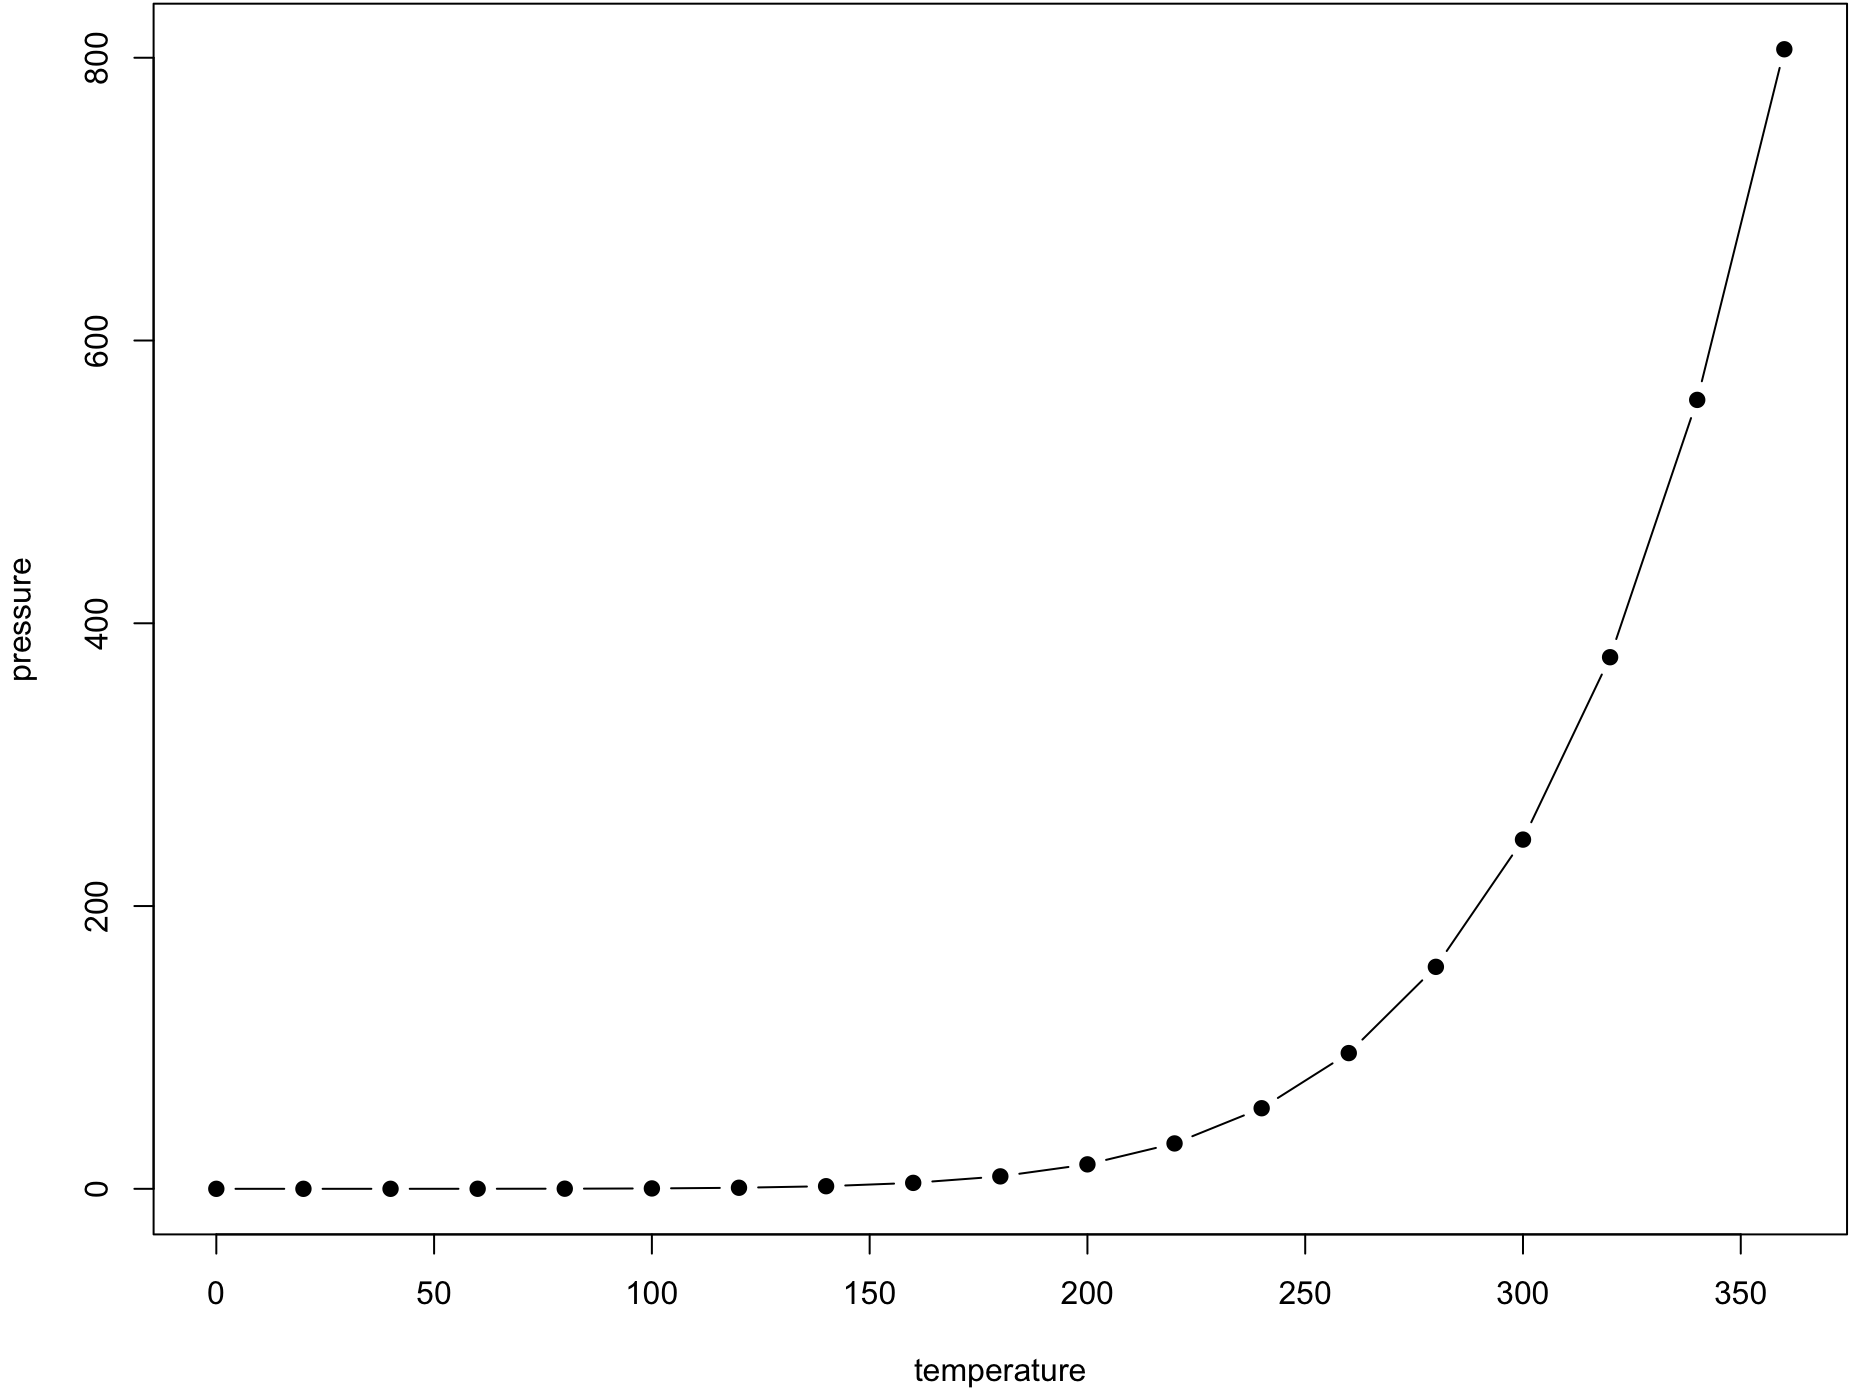
\includegraphics[width=0.8\linewidth]{figures/nice-fig-1} 

}

\caption{Here is a nice figure!}\label{fig:nice-fig}
\end{figure}

Reference a figure by its code chunk label with the \texttt{fig:} prefix, e.g., see Figure \ref{fig:nice-fig}. Similarly, you can reference tables generated from \texttt{knitr::kable()}, e.g., see Table \ref{tab:nice-tab}.

\begin{table}

\caption{\label{tab:nice-tab}Here is a nice table!}
\centering
\begin{tabular}[t]{rrrrl}
\toprule
Sepal.Length & Sepal.Width & Petal.Length & Petal.Width & Species\\
\midrule
5.1 & 3.5 & 1.4 & 0.2 & setosa\\
4.9 & 3.0 & 1.4 & 0.2 & setosa\\
4.7 & 3.2 & 1.3 & 0.2 & setosa\\
4.6 & 3.1 & 1.5 & 0.2 & setosa\\
5.0 & 3.6 & 1.4 & 0.2 & setosa\\
\addlinespace
5.4 & 3.9 & 1.7 & 0.4 & setosa\\
4.6 & 3.4 & 1.4 & 0.3 & setosa\\
5.0 & 3.4 & 1.5 & 0.2 & setosa\\
4.4 & 2.9 & 1.4 & 0.2 & setosa\\
4.9 & 3.1 & 1.5 & 0.1 & setosa\\
\addlinespace
5.4 & 3.7 & 1.5 & 0.2 & setosa\\
4.8 & 3.4 & 1.6 & 0.2 & setosa\\
4.8 & 3.0 & 1.4 & 0.1 & setosa\\
4.3 & 3.0 & 1.1 & 0.1 & setosa\\
5.8 & 4.0 & 1.2 & 0.2 & setosa\\
\addlinespace
5.7 & 4.4 & 1.5 & 0.4 & setosa\\
5.4 & 3.9 & 1.3 & 0.4 & setosa\\
5.1 & 3.5 & 1.4 & 0.3 & setosa\\
5.7 & 3.8 & 1.7 & 0.3 & setosa\\
5.1 & 3.8 & 1.5 & 0.3 & setosa\\
\bottomrule
\end{tabular}
\end{table}

You can write citations, too. For example, we are using the \textbf{bookdown} package \citep{R-bookdown} in this sample book, which was built on top of R Markdown and \textbf{knitr} \citep{xie2015}.

\hypertarget{core-theory}{%
\chapter{Core theory}\label{core-theory}}

\hypertarget{principles-of-data-science}{%
\section{Principles of data science}\label{principles-of-data-science}}

\hypertarget{what-is-data-science}{%
\subsection{What is data science?}\label{what-is-data-science}}

\hypertarget{what-is-the-data-life-cycle}{%
\subsection{What is the data life cycle?}\label{what-is-the-data-life-cycle}}

\hypertarget{what-is-a-pipeline}{%
\subsection{What is a pipeline?}\label{what-is-a-pipeline}}

\hypertarget{data-science-in-the-wild}{%
\subsection{Data science `in the wild'}\label{data-science-in-the-wild}}

\hypertarget{the-reproducibility-crisis}{%
\subsection{The reproducibility crisis}\label{the-reproducibility-crisis}}

\hypertarget{data-ethics-and-citizenship}{%
\section{Data, ethics, and citizenship}\label{data-ethics-and-citizenship}}

\hypertarget{principles-of-data-visualization}{%
\section{Principles of data visualization}\label{principles-of-data-visualization}}

\hypertarget{bad-examples}{%
\subsection{Bad examples}\label{bad-examples}}

\hypertarget{good-exaples}{%
\subsection{Good exaples}\label{good-exaples}}

\hypertarget{edward-tufte}{%
\subsection{Edward Tufte}\label{edward-tufte}}

\hypertarget{grammar-of-graphics}{%
\subsection{Grammar of graphics}\label{grammar-of-graphics}}

\hypertarget{design-principles}{%
\subsection{Design principles}\label{design-principles}}

\hypertarget{plots-power-the-politics-of-plotting}{%
\subsection{Plots \& power: the politics of plotting}\label{plots-power-the-politics-of-plotting}}

\hypertarget{principles-of-data-writing}{%
\section{Principles of data writing}\label{principles-of-data-writing}}

\hypertarget{getting-started-in-r}{%
\chapter{Getting started in R}\label{getting-started-in-r}}

\hypertarget{downloading-r-and-rstudio}{%
\section{Downloading R and RStudio}\label{downloading-r-and-rstudio}}

\hypertarget{running-r-code-basic-math-operators}{%
\section{Running R code: basic math \& operators}\label{running-r-code-basic-math-operators}}

\hypertarget{rstudio-tour-workflow-scripts}{%
\section{RStudio: Tour, workflow, \& scripts}\label{rstudio-tour-workflow-scripts}}

\hypertarget{objects-variables-and-vectors}{%
\section{Objects: variables and vectors}\label{objects-variables-and-vectors}}

\hypertarget{calling-functions}{%
\section{Calling functions}\label{calling-functions}}

\hypertarget{base-plots}{%
\section{Base plots}\label{base-plots}}

\hypertarget{packages}{%
\section{Packages}\label{packages}}

\hypertarget{ggplot}{%
\section{ggplot}\label{ggplot}}

\hypertarget{working-with-data-in-r}{%
\chapter{Working with data in R}\label{working-with-data-in-r}}

\hypertarget{project-workflows}{%
\section{Project workflows}\label{project-workflows}}

\hypertarget{importing-data}{%
\section{Importing data}\label{importing-data}}

\hypertarget{working-directories}{%
\subsection{Working directories}\label{working-directories}}

\hypertarget{reading-in-data}{%
\subsection{Reading in data}\label{reading-in-data}}

\hypertarget{dataframes-exploration-summarization}{%
\section{Dataframes: exploration \& summarization}\label{dataframes-exploration-summarization}}

\hypertarget{data-wrangling}{%
\section{Data wrangling}\label{data-wrangling}}

\hypertarget{data-transformation-filtering-grouping}{%
\subsection{Data transformation, filtering, \& grouping}\label{data-transformation-filtering-grouping}}

\hypertarget{the-tidyverse-and-tibbles}{%
\subsection{The tidyverse and tibbles}\label{the-tidyverse-and-tibbles}}

\hypertarget{transformation-with-dplyr}{%
\subsection{Transformation with dplyr}\label{transformation-with-dplyr}}

\hypertarget{exploratory-data-analysis}{%
\section{Exploratory Data Analysis}\label{exploratory-data-analysis}}

\hypertarget{exploring-distributions}{%
\subsection{Exploring distributions}\label{exploring-distributions}}

\hypertarget{variable-types-statistics}{%
\subsection{Variable types \& statistics}\label{variable-types-statistics}}

\hypertarget{descriptive-statistics}{%
\subsection{Descriptive statistics}\label{descriptive-statistics}}

\hypertarget{significance-statistics}{%
\section{Significance statistics}\label{significance-statistics}}

\hypertarget{comparison-tests}{%
\subsection{Comparison tests}\label{comparison-tests}}

\hypertarget{correlation-tests}{%
\subsection{Correlation tests}\label{correlation-tests}}

\hypertarget{customizing-plots}{%
\section{Customizing plots}\label{customizing-plots}}

\hypertarget{base-plots-1}{%
\subsection{Base plots}\label{base-plots-1}}

\hypertarget{ggplot-1}{%
\subsection{ggplot}\label{ggplot-1}}

\hypertarget{managing-project-files}{%
\section{Managing project files}\label{managing-project-files}}

\hypertarget{formatting-your-own-data}{%
\section{Formatting your own data}\label{formatting-your-own-data}}

\hypertarget{your-core-r-toolkit}{%
\chapter{Your core R toolkit}\label{your-core-r-toolkit}}

\hypertarget{uniting-and-joining-data}{%
\section{Uniting and joining data}\label{uniting-and-joining-data}}

\hypertarget{for-loops}{%
\section{For loops}\label{for-loops}}

\hypertarget{writing-functions}{%
\section{Writing functions}\label{writing-functions}}

\hypertarget{working-with-text}{%
\section{Working with text}\label{working-with-text}}

\hypertarget{cleaning-messy-data}{%
\section{Cleaning messy data}\label{cleaning-messy-data}}

\hypertarget{working-with-factors}{%
\section{Working with factors}\label{working-with-factors}}

\hypertarget{matrices-lists}{%
\section{Matrices \& lists}\label{matrices-lists}}

\hypertarget{pipes}{%
\section{Pipes}\label{pipes}}

\hypertarget{exporting-data-plots}{%
\section{Exporting data \& plots}\label{exporting-data-plots}}

\hypertarget{web-based-data}{%
\section{Web-based data}\label{web-based-data}}

\hypertarget{interactive-dashboards-in-r}{%
\chapter{Interactive dashboards in R}\label{interactive-dashboards-in-r}}

\hypertarget{shiny-dashboards}{%
\section{Shiny dashboards}\label{shiny-dashboards}}

\hypertarget{data-entry-apps}{%
\section{Data entry apps}\label{data-entry-apps}}

\hypertarget{databases}{%
\chapter{Databases}\label{databases}}

\hypertarget{intro-what-why-when-and-when-not}{%
\section{Intro: What, why, when (and when not)}\label{intro-what-why-when-and-when-not}}

\hypertarget{platforms-postgresql-mysql-sqlite-etc.}{%
\section{Platforms: PostgreSQL, mySQL, SQLite, etc.}\label{platforms-postgresql-mysql-sqlite-etc.}}

\hypertarget{alternatives-nosql}{%
\section{Alternatives: NoSQL}\label{alternatives-nosql}}

\hypertarget{practical-spinning-up-a-local-db}{%
\section{Practical: spinning up a local DB}\label{practical-spinning-up-a-local-db}}

\hypertarget{reproducible-research-documentation-in-r}{%
\chapter{Reproducible research \& documentation in R}\label{reproducible-research-documentation-in-r}}

\hypertarget{introduction-to-rmarkdown}{%
\section{Introduction to Rmarkdown}\label{introduction-to-rmarkdown}}

\hypertarget{standards-for-tables}{%
\section{Standards for tables}\label{standards-for-tables}}

\hypertarget{standards-for-figures}{%
\section{Standards for figures}\label{standards-for-figures}}

\hypertarget{version-control-and-teamwork}{%
\chapter{Version control and teamwork}\label{version-control-and-teamwork}}

\hypertarget{what-is-version-control}{%
\section{What is version control?}\label{what-is-version-control}}

\hypertarget{github}{%
\section{Github}\label{github}}

\hypertarget{standard-git-operations}{%
\section{Standard git operations}\label{standard-git-operations}}

\hypertarget{other-git-platforms}{%
\section{Other git platforms}\label{other-git-platforms}}

\hypertarget{scientific-writing-techniques}{%
\chapter{Scientific writing techniques}\label{scientific-writing-techniques}}

\hypertarget{advanced-skills}{%
\chapter{Advanced skills}\label{advanced-skills}}

\hypertarget{geographic-computing-gis}{%
\section{Geographic computing \& GIS}\label{geographic-computing-gis}}

\hypertarget{mapping}{%
\section{Mapping}\label{mapping}}

\hypertarget{statistical-modeling}{%
\section{Statistical modeling}\label{statistical-modeling}}

\hypertarget{apply-family}{%
\section{Apply family}\label{apply-family}}

\hypertarget{iterative-analyses}{%
\section{Iterative analyses}\label{iterative-analyses}}

\hypertarget{randomization}{%
\subsection{Randomization}\label{randomization}}

\hypertarget{simulations}{%
\subsection{Simulations}\label{simulations}}

  \bibliography{book.bib,packages.bib}

\end{document}
